\clearpage
\subsection{Implementation view}
\copied{The development view illustrates a system from a programmer's perspective and is concerned with software management. This view is also known as the implementation view. It uses the UML Component diagram to describe system components. UML Diagrams used to represent the development view include the Package diagram.}
{from wikipedia\\\url{https://en.wikipedia.org/wiki/4\%2B1_architectural_view_model}}

The implementation view, also known as the development view, describes the system from the programmer's perspective. This includes a description of the components of the system and how the system is packaged.  

\subsubsection{Components}
The system consists of a set of components tat all interact with each other. In figure~\ref{fig:component} below, these different components are shown. Each component can provide interfaces and uses sockets to connect to interfaces of other components. This way, the implementation of each component can independently be replaced and deployed. 

\clearpage
\begin{figure}[h]
%\centering
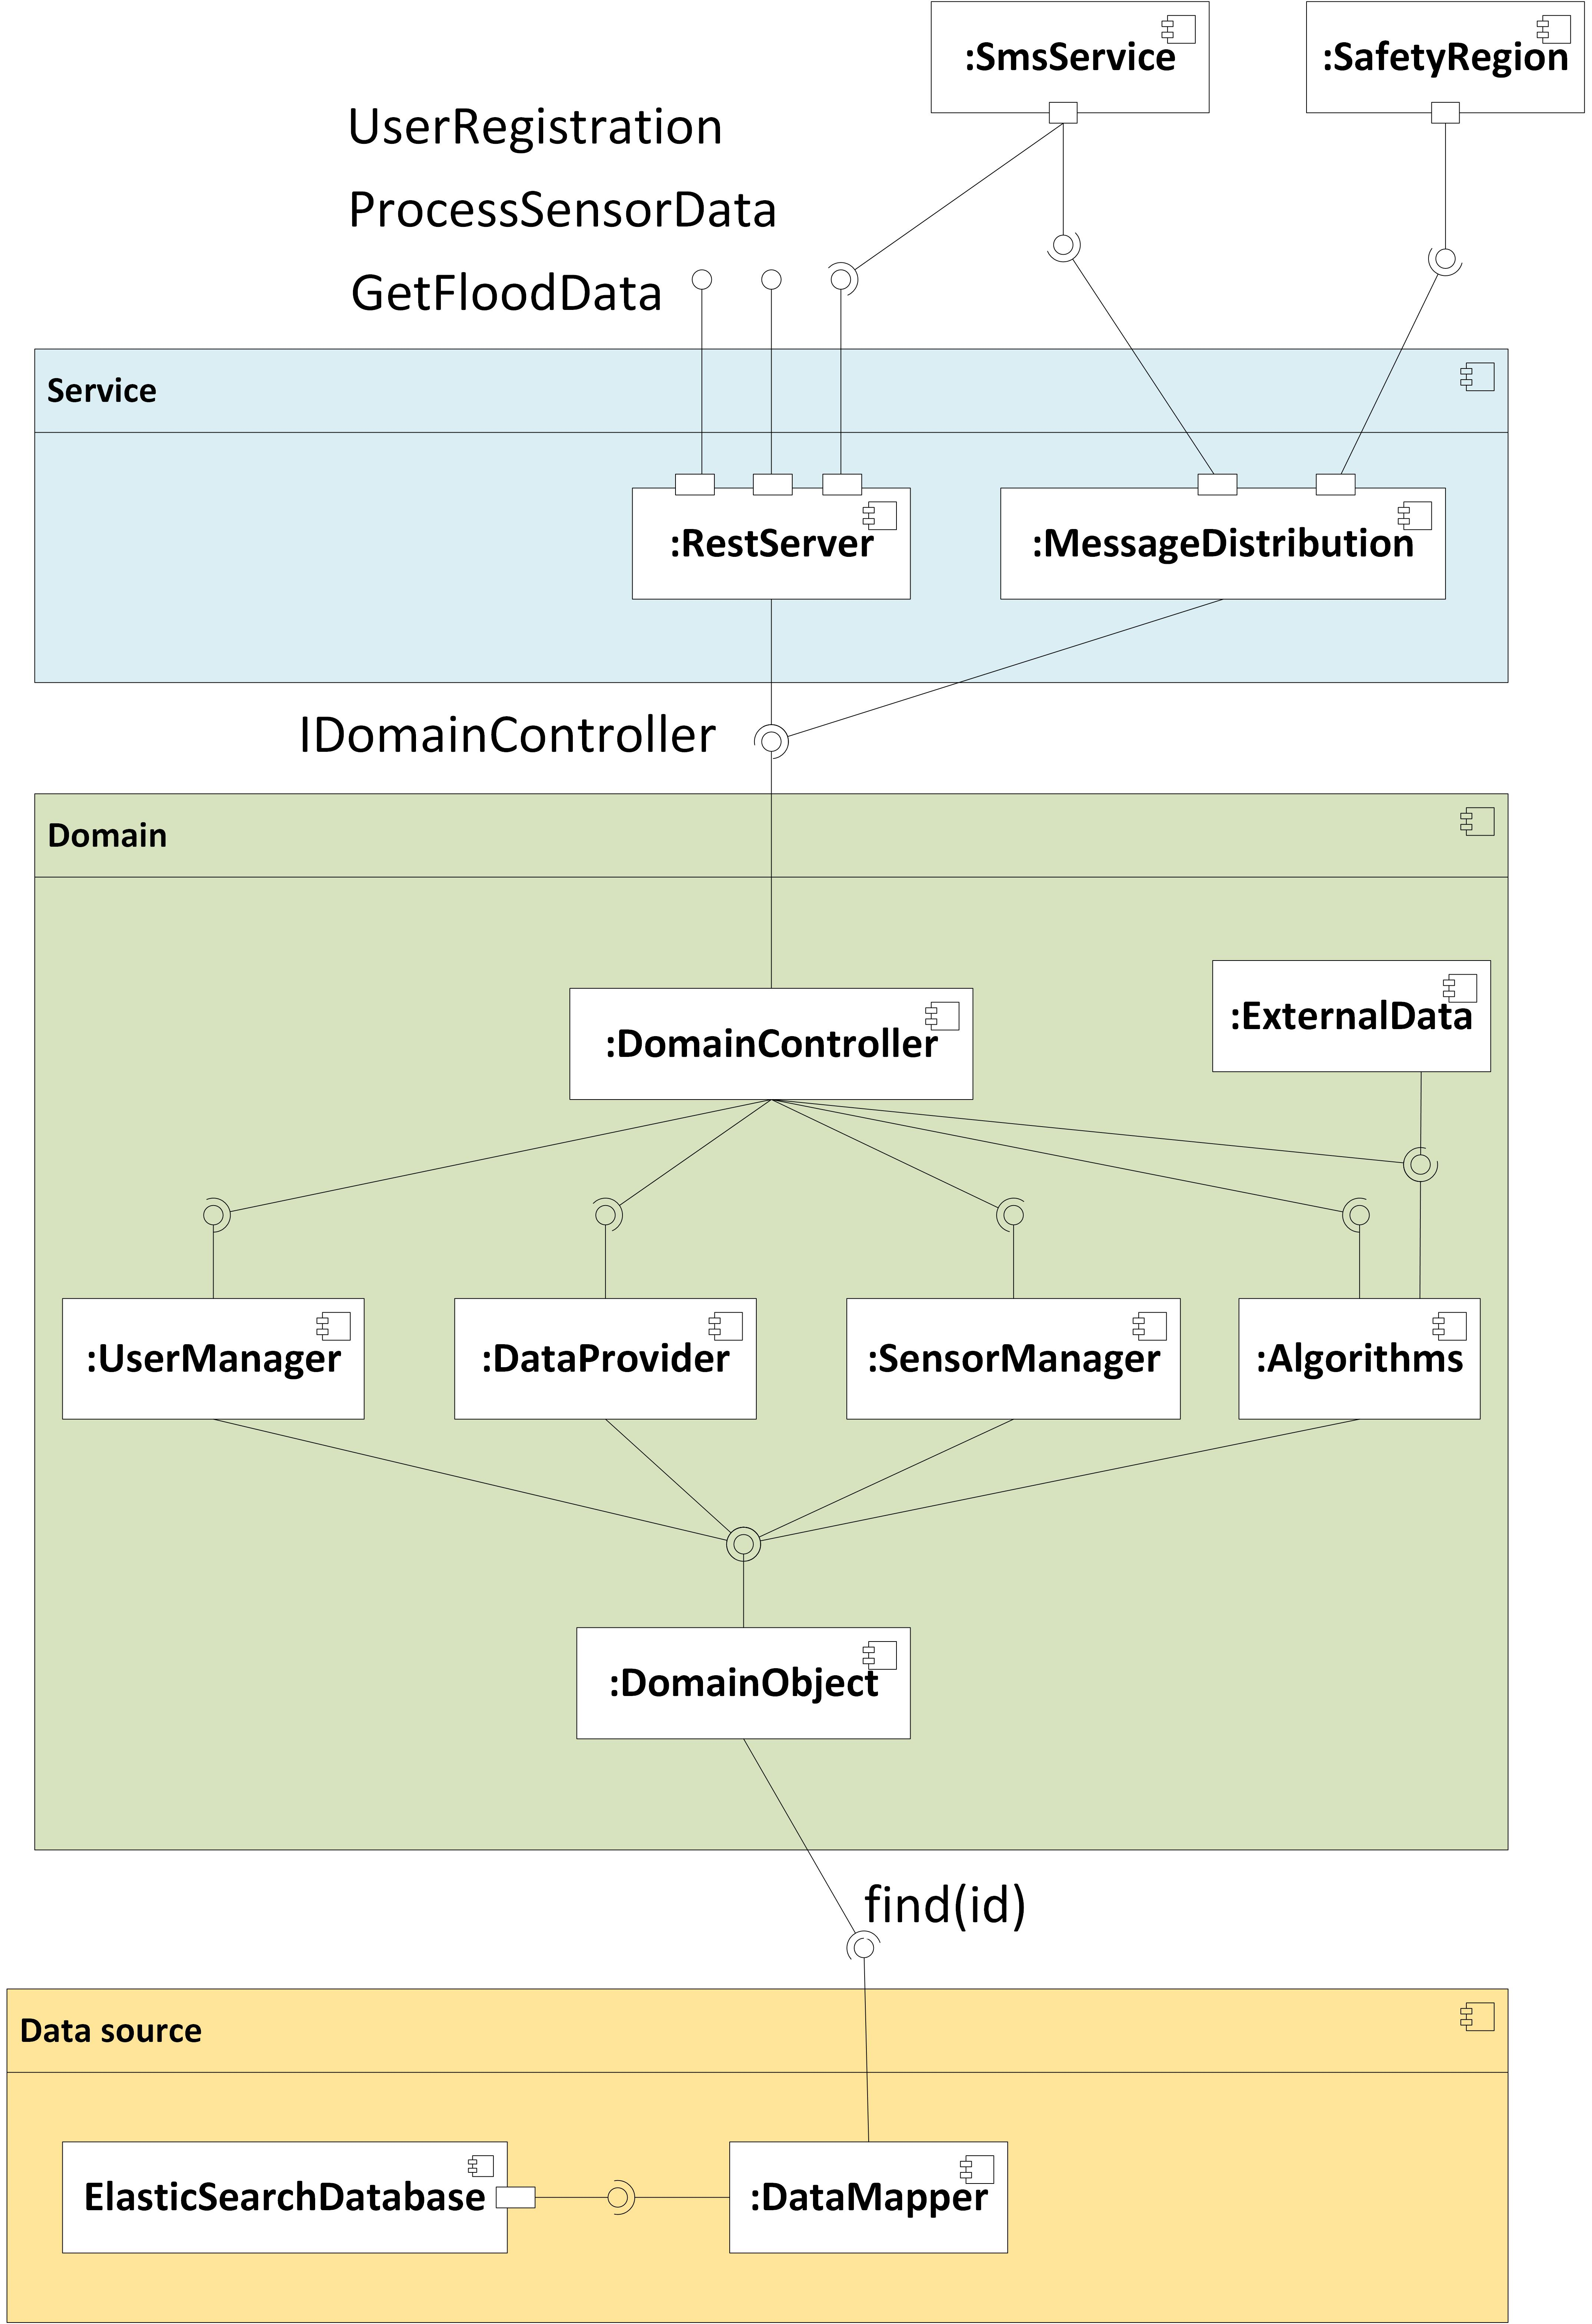
\includegraphics[keepaspectratio=true,height=13cm,width=0.9\textwidth]{{\viewimages/component}.jpg}
\caption{Component diagram}
\label{fig:component}
\end{figure}

\todo{explain the components}

\subsection{Database}
The figure \ref{fig:database} below shows how the database is structured. 

\clearpage
\begin{figure}[hb!]
%\centering
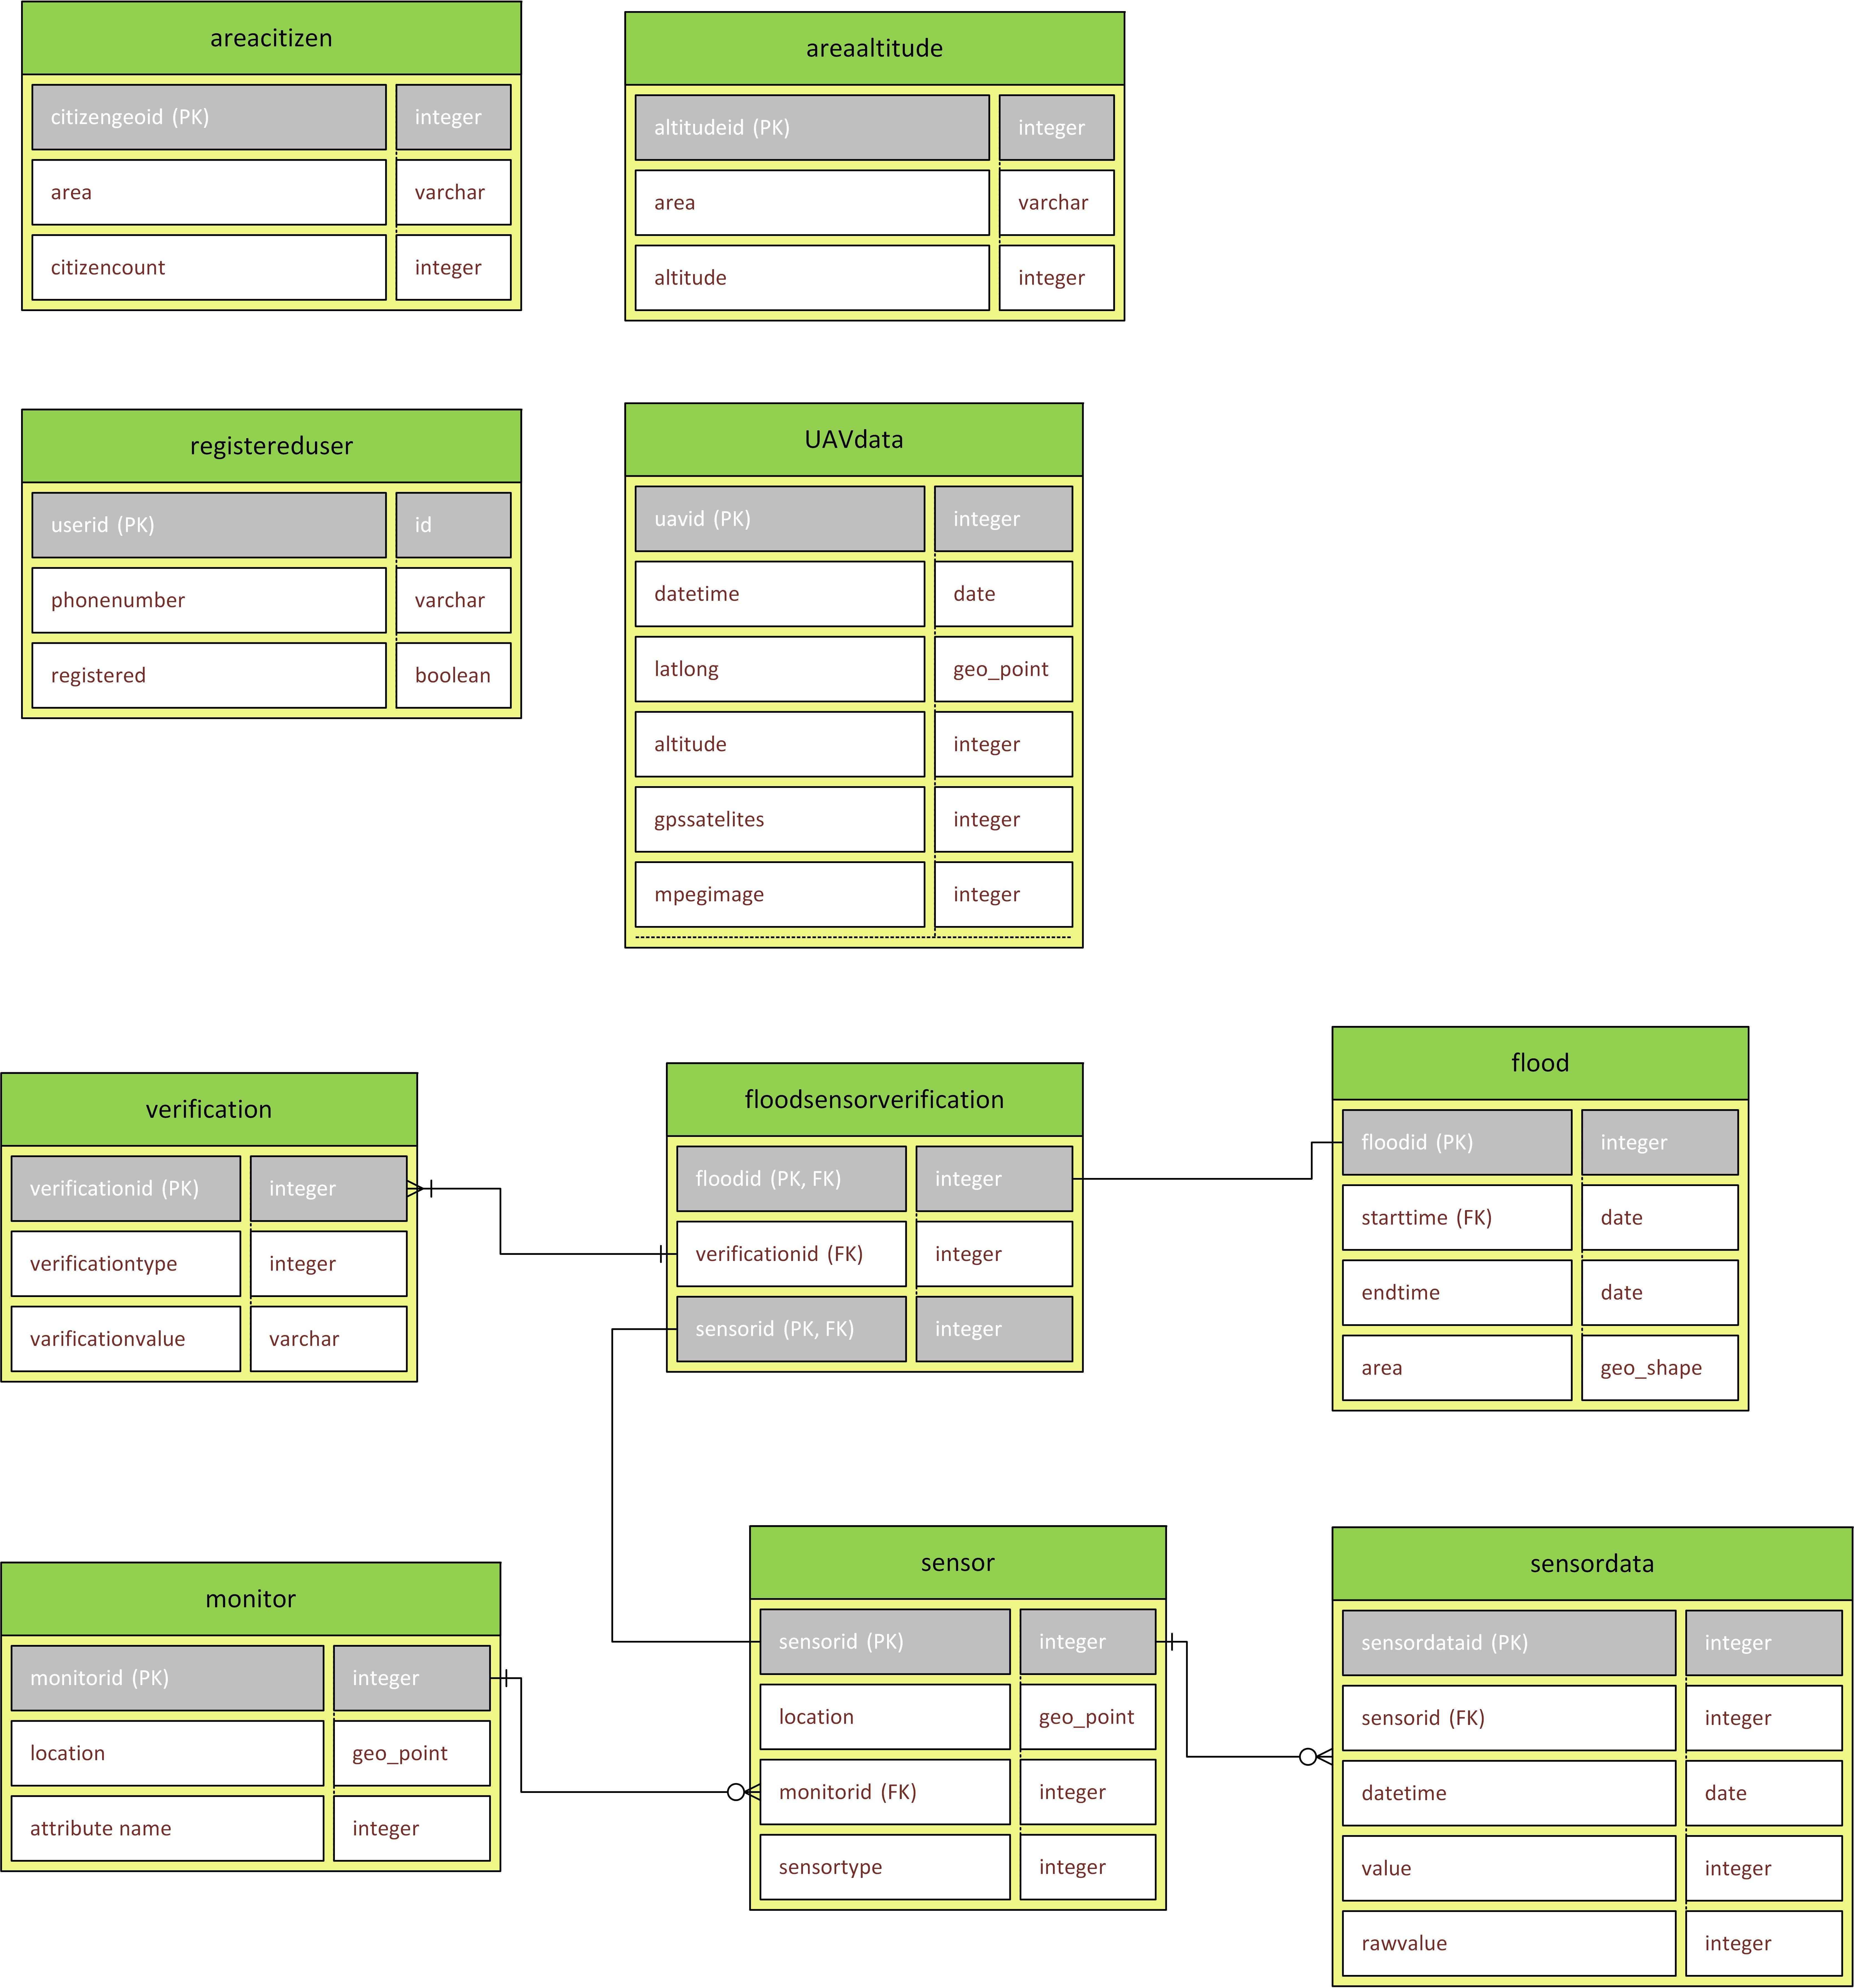
\includegraphics[height=14cm, width=0.9\textwidth]{{\viewimages/database}.jpg}
\caption{Database diagram}
\label{fig:database}
\end{figure}

The database diagram shows all the information the API can provide to the users. \\
The database is made of ten tables. \\

In green is the name of the table. \\
In grey the primarykey. \\
In the second column of each table are the types of the data. \\

The first table \textbf{aeracitizen} concerns the area where live the citizens : citizengeold (?) , area : the name of the area and citizencount gives the number of citizen in this area.\\
 The table \textbf{aeraaltitude} gives information about the are such as its altitude.
The table \textbf{UAVdata} provides information sent by the UAVs which will give more information about the flood such as : uavid which identifies a specific uav, datetime, altitude , latlong ,gpssatelite,mpegimage, \\
The table \textbf{registereduser} concerns information to identify a specific user to provide him the warning, provide guidance and help the safety region : his id, phonenumer and if he is registered or not. \\

Six table are related and provide information about the sensors : \\
verification (?) \\
The table \textbf{Floodsensorverification} (?) \\
The table \textbf{flood}gives information about the flood : its id by floodid , starttime , endtimide , area. \\
The table \textbf{monitor} : monitorid , its location, attributename. \\
The table \textbf{sensor} : sensorid identifies each sensor, its location , which monitor it depends on,and its type \\
The table \textbf{sensordata} : sensordataid which identifies each data of the sensor, sensorid, datetime which gives the exact time of when the data has been sent ,value,  rawvalue(?). 

\subsubsection{Packages}
The software of the system is divided into several packages. These packages and their relations can be seen in figure~\ref{fig:package-diagram}. 
In this diagram, «use» depicts the use of an interface exposed by a software package, «access» depicts a private import of (parts of) another package, while «import» means a public import of (parts of) another package. 

The diagram contains software packages of the system itself, as well as software packages provided by third parties. The software packages provided by third parties are drawn outside of the `Smart Flood Monitoring System'-box.

The `Third Party API' is the software package which exposes a REST-API, which can be used by third parties to query data from the system.
The `External Data' is the software package which uses APIs from other systems to query data, like weather and geographic data.

\begin{figure}[h]
%\centering
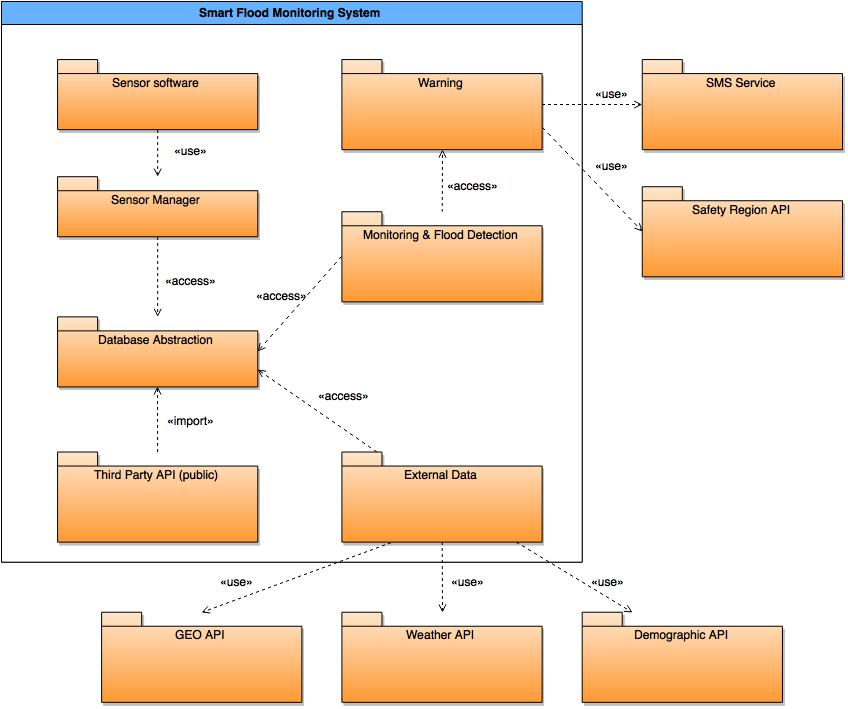
\includegraphics[keepaspectratio=true,width=1.0\textwidth]{{\viewimages/packages}.png}
\caption{Package diagram}
\label{fig:package-diagram}
\end{figure}